\cleardoublepage

\section{国内外研究现状}
\par 目前国内外通过计算机辅助医生进行宫颈TCT检测的方法主要分为病变细胞分类、病变细胞检测、病变部位分割三个部分。
\par 病变细胞分类主要是指仅给出输入视野中细胞的综合病变等级,一般会根据病变细胞的状况评定为在视野中出现的最高病变等级或者次高级。

\begin{figure}[h]
    \centering
    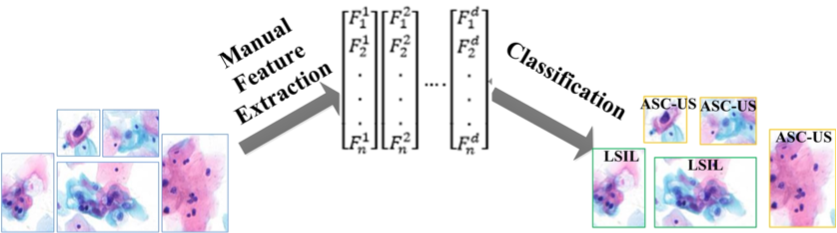
\includegraphics[width=0.5\paperwidth]{TCT/分类样例.png}
    \caption{病变细胞分类样例图片,输入图片经过提取特征等处理后由计算机判断图片所属的病变等级}
    \label{pic:分类样例}
\end{figure}
\par 病变细胞检测则是要求以矩形框的方式标注出视野内的病变细胞并给出病变等级,相较病变细胞分类任务而言,评定整个视野的综合病变等级的任务由医生完成。在病变细胞检测的任务中,计算机应当标注出所有病变细胞的位置并给每个病变细胞评定病变等级。

\begin{figure}[h]
    \centering
    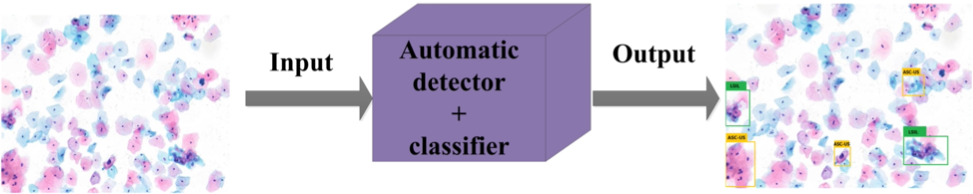
\includegraphics[width=0.5\paperwidth]{TCT/检测样例.png}
    \caption{病变细胞检测样例图片,输入图片经过提取特征等处理后由计算机检测图片所有的病变细胞并判定其所属的病变等级}
    \label{pic:检测样例}
\end{figure}
\par 病变细胞分割则是在病变细胞检测的基础上,要求以像素级的精度标注出病变细胞的范围。病变细胞分割的任务中,计算机标注病变细胞位置的结果应当更为精确。

\begin{figure}[h]
    \centering
    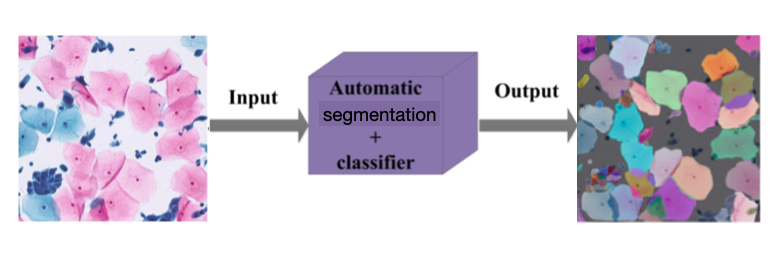
\includegraphics[width=0.5\paperwidth]{TCT/分割样例.png}
    \caption{分割样例图片,左图为样例图片,右图为样例图片的分割结果}
    \label{pic:分割样例}
\end{figure}

\subsection{病变细胞分类与分割}
\par 在临床实践中,医生主要依据细胞核与细胞质的比例,细胞核的大小,细胞核的形状以及核膜的异常变化来判定病变的宫颈细胞,以及区分它们的种类。因此,有许多研究\cite{zhang2014segmentation}\cite{zhang2017graph}\cite{lee2016segmentation}通过分割细胞或细胞的某些部分(细胞核、细胞质),并依据临床上的判定规则完成病变细胞的分类任务。但是由于不同种类细胞的形态差异较大、细胞之间的重叠问题可能比较严重以及细胞质边界可能不够清晰等问题,细胞以及细胞成分的分割依然是一个尚未被很好解决的问题。因此,这类方法往往不能让人满意。
\par 而在另一方面,也有许多研究\cite{marinakis2009pap}\cite{phoulady2016automatic}通过手工设计大量的特征试图捕捉细胞核和细胞质的形态特征,再将这些特征经过特征选择或者降维处理之后输入到各种分类器中(如,随机森林、SVM、神经网络等)来完成分类任务。但是,上述的手工设计的特征往往依赖于细胞或细胞组成成分的分割结果,而且这些手工设计的特征完全来自于当前医学对于宫颈细胞学的认知,因此,此类方法的发展会受到医学发展的限制。
\subsection{病变细胞检测}
\par 近期,病变细胞检测方向的研究主要是基于卷积神经网络进行的。例如,Ma等\cite{ma2020macd}中设计了新的MACD R-CNN网络,通过在Mask R-CNN的不同分类分支中使用不同的roi提取出一个细胞核特征变形的特征图,将这种特征图与固定roi的特征通过注意力机制合并,最后通过加入更深的卷积层深度提高了检测的精度;Xiang等\cite{xiang2020novel}基于YOLOv3级联了一个额外的特定任务分类器,还通过平滑噪声标签的分布来处理可能存在的不可靠标注,最终提高了宫颈细胞水平诊断的平均精度;Liang等\cite{liang2018comparison}通过将图像提案与各类别的参考样本进行比较,来对图像提案进行分类,并且从数据中学习背景的参考样本,而不是通过一些启发式规则手工选择参考样本,这种方法在小数据集上相较与基准模型会有明显提升,在中等数据集上会略有提升;Li等\cite{li2019detection}提出了一种基于多语义标签和形态信息分析相结合的目标检测和分类方法,该方法以ResNet101作为骨干网络时可以在LBC数据集上取得66.98\%的平均精度;Liu等\cite{liu2018multitask}使用VGG16迁移学习,并用一种面向任务的基于先验框的网络将产生潜在的感兴趣区域,最后使用全卷积网络来估计细胞的位置并将其分类,这种方法在保持性能和计算效率之间取得了良好的平衡,相较于YOLO和Faster R-CNN它拥有更好的精度和更快的速度,例如,这种方法的耗时只有Faster R-CNN的一半。
\par 除此之外,由于卷积神经网络的学习往往需要大量的标注数据,而TCT图像的标注结果是由专业的医师来完成的,那么获取大量的数据就会带来高额的成本,因此也有许多研究\cite{zhou2020deep}\cite{yu2019uncertainty}通过一些半监督的方法来利用大量无标注信息的图像促进网络的学习。Zhou等\cite{zhou2020deep}提出了一种新的带扰动敏感样本挖掘的掩码引导的均值教师框架,该框架在训练过程中由教师和学生网络组成。在小扰动条件下,两个网络在特征和语义层面上保持一致。从教师网络对样本的预测来构建可靠的伪标签以优化学生网络。他们设计了一个新的策略来估计每个提案对扰动的敏感性,并从大量的可能样本中选择最具信息量的样本,以促进快速有效的语义提取。此外,为了消除背景区域不可避免的噪声,他们希望以预测出的分割掩模作为指导以加强前景区域的特征蒸馏。与仅使用已有标注数据的监督方法相比,该方法的性能有显著提高;Yu等\cite{yu2019uncertainty}提出了一种新的不确定性感知的半监督框架,该框架可以有效地利用未标记的数据,鼓励在不同扰动下对相同输入进行一致的预测。具体来说,该框架由一个学生模型和一个教师模型组成,学生模型通过最小化分割损失和一致性损失对教师模型的目标进行学习。他们设计了一种新的不确定性感知方案,使学生模型能够利用不确定性信息逐步学到有意义的、可靠的目标。实验表明,该方法通过合并未标记的数据获得了较高的性能。
\par 目前病变细胞检测方面相关的论文、其所使用的方法、数据集以及最终效果(部分)如\ref{tab:检测论文}:
\begin{table}[htbp]
    \center
    \tiny
    \caption{病变细胞检测论文汇总}
    \begin{tabular}{p{120pt}p{100pt}p{85pt}p{35pt}}
        \hline
        论文                                                             & 模型                         & 数据                       & 效果(mAP) \\
        \hline
        MACD R-CNN\cite{ma2020macd}                                      & 基于mask R-CNN 的 MACD R-CNN & Herlev 数据集              & -           \\
        Automation-Assisted Reading Method\cite{xiang2020novel}          & YOLO V3 和额外的分类器       & 私有数据12909 例,10个类别 & 0.634       \\
        Detection in the Limited Data Scenario\cite{liang2018comparison} & Faster R-CNN + FPN           & 私有数据7086例,11个类别   & 0.263       \\
        Detection and Classification of Cells\cite{li2019detection}      & Faster R-CNN                 & 680例,6个类别             & -           \\
        Multitask Learning for Recognition\cite{liu2018multitask}        & VGG16                        & 73 例                      & -           \\
        DCCL\cite{zhang2019dccl}                                         & Faster R-CNN,RetinaNet      & DCCL公开数据               & -           \\
        \hline
    \end{tabular}
    \label{tab:检测论文}
\end{table}

\section{数据集}
\par 我们的数据集拥有6957张图片,包含ASCUS(非典型鳞状细胞意义不明确)、LSIL(低度鳞状上皮内病变)、ASCH(非典型鳞状细胞不排除高级别鳞状上皮内病变)、HSIL(高度鳞状上皮内病变)、SQCA(鳞状上皮癌)五种病变类别,以及NORMAL(正常细胞)一种正常类别。各类别标注框的数量与含有该类别的图片的数量如表\ref{tab:类别}所示。

\begin{table}[htbp]
    \center
    \caption{各类别标注框数量与图片数量}
    \begin{tabular}{cccc}
        \hline
        类别 & 标注框数量 & 图片数量 \\
        \hline
        ASCUS & 4065 & 2635 \\
        LSIL & 3241 & 2323 \\
        ASCH & 1357 & 946 \\
        HSIL & 13001 & 2771 \\
        SQCA & 390 & 124 \\
        NORMAL & 4796 & 2872 \\
        \hline
    \end{tabular}
    \label{tab:类别}
\end{table}

部分数据集中图片与标注框的可视化如图\ref{pic:数据集可视化}所示。
\begin{figure}[htb]
    \centering
    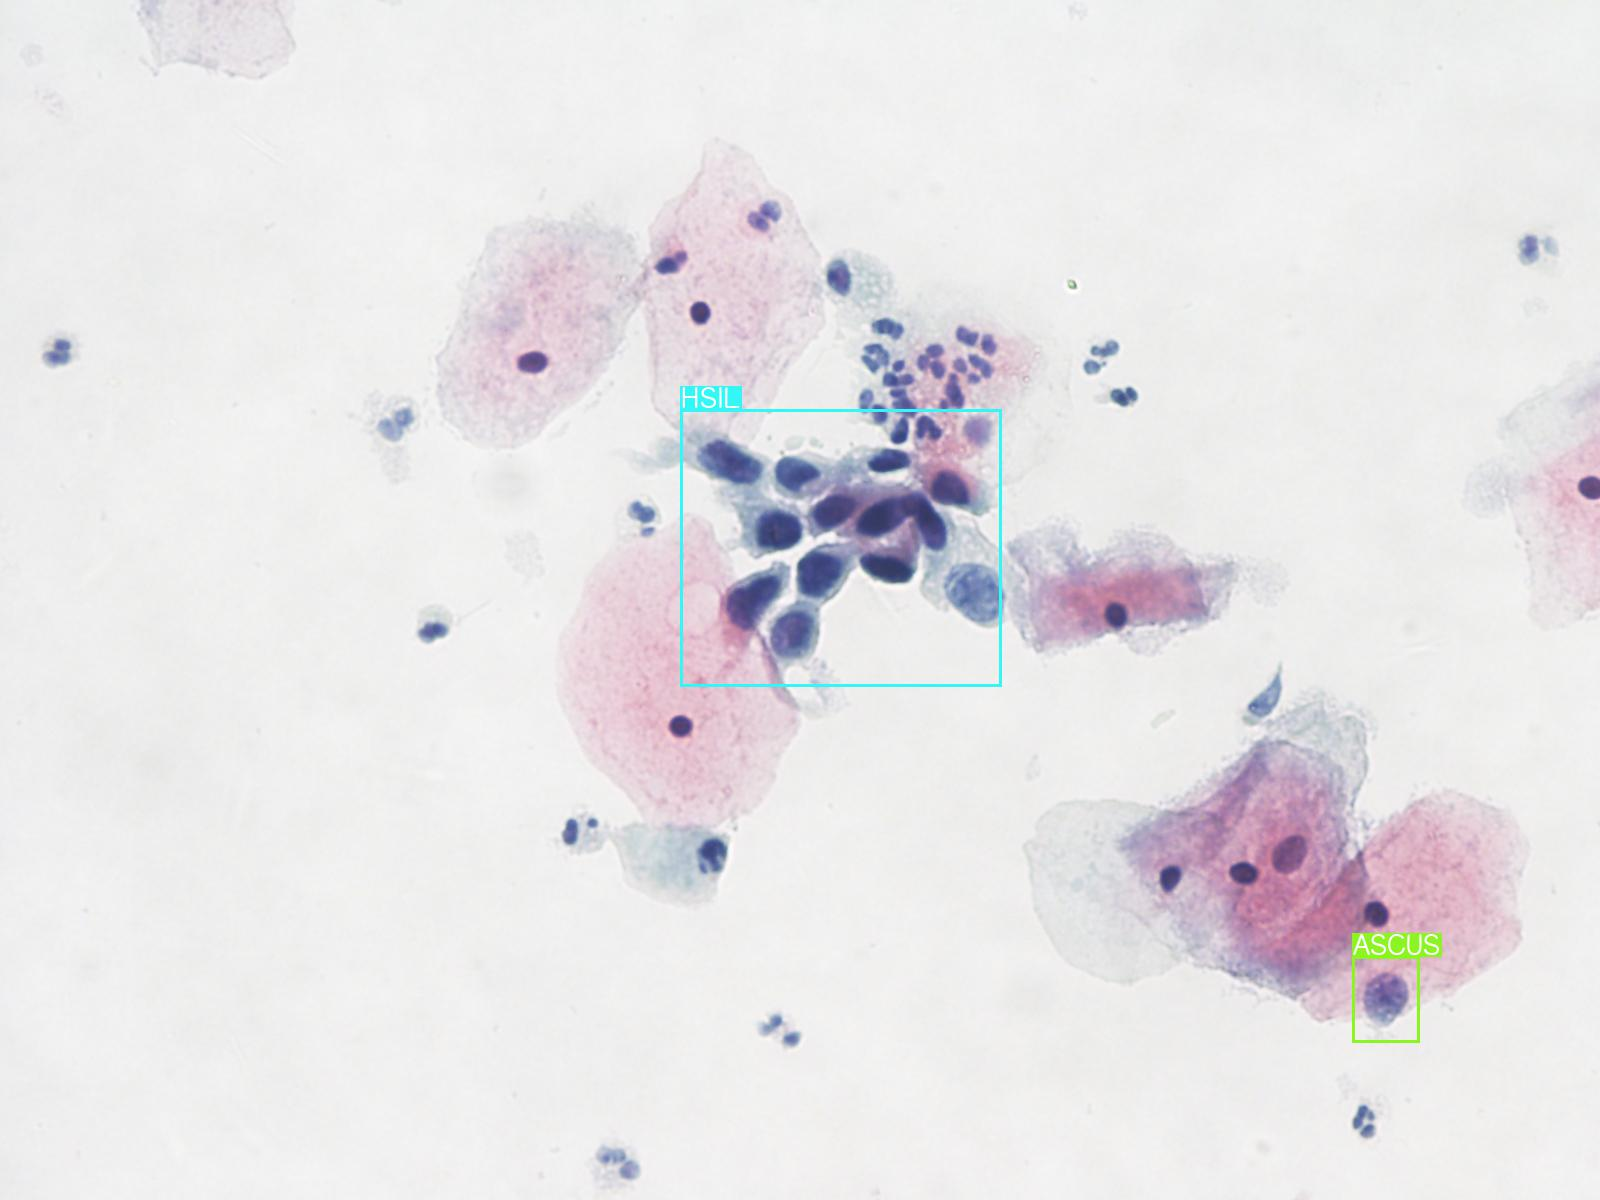
\includegraphics[width = .49\linewidth]{TCTDataSet/可视化1.jpg}
    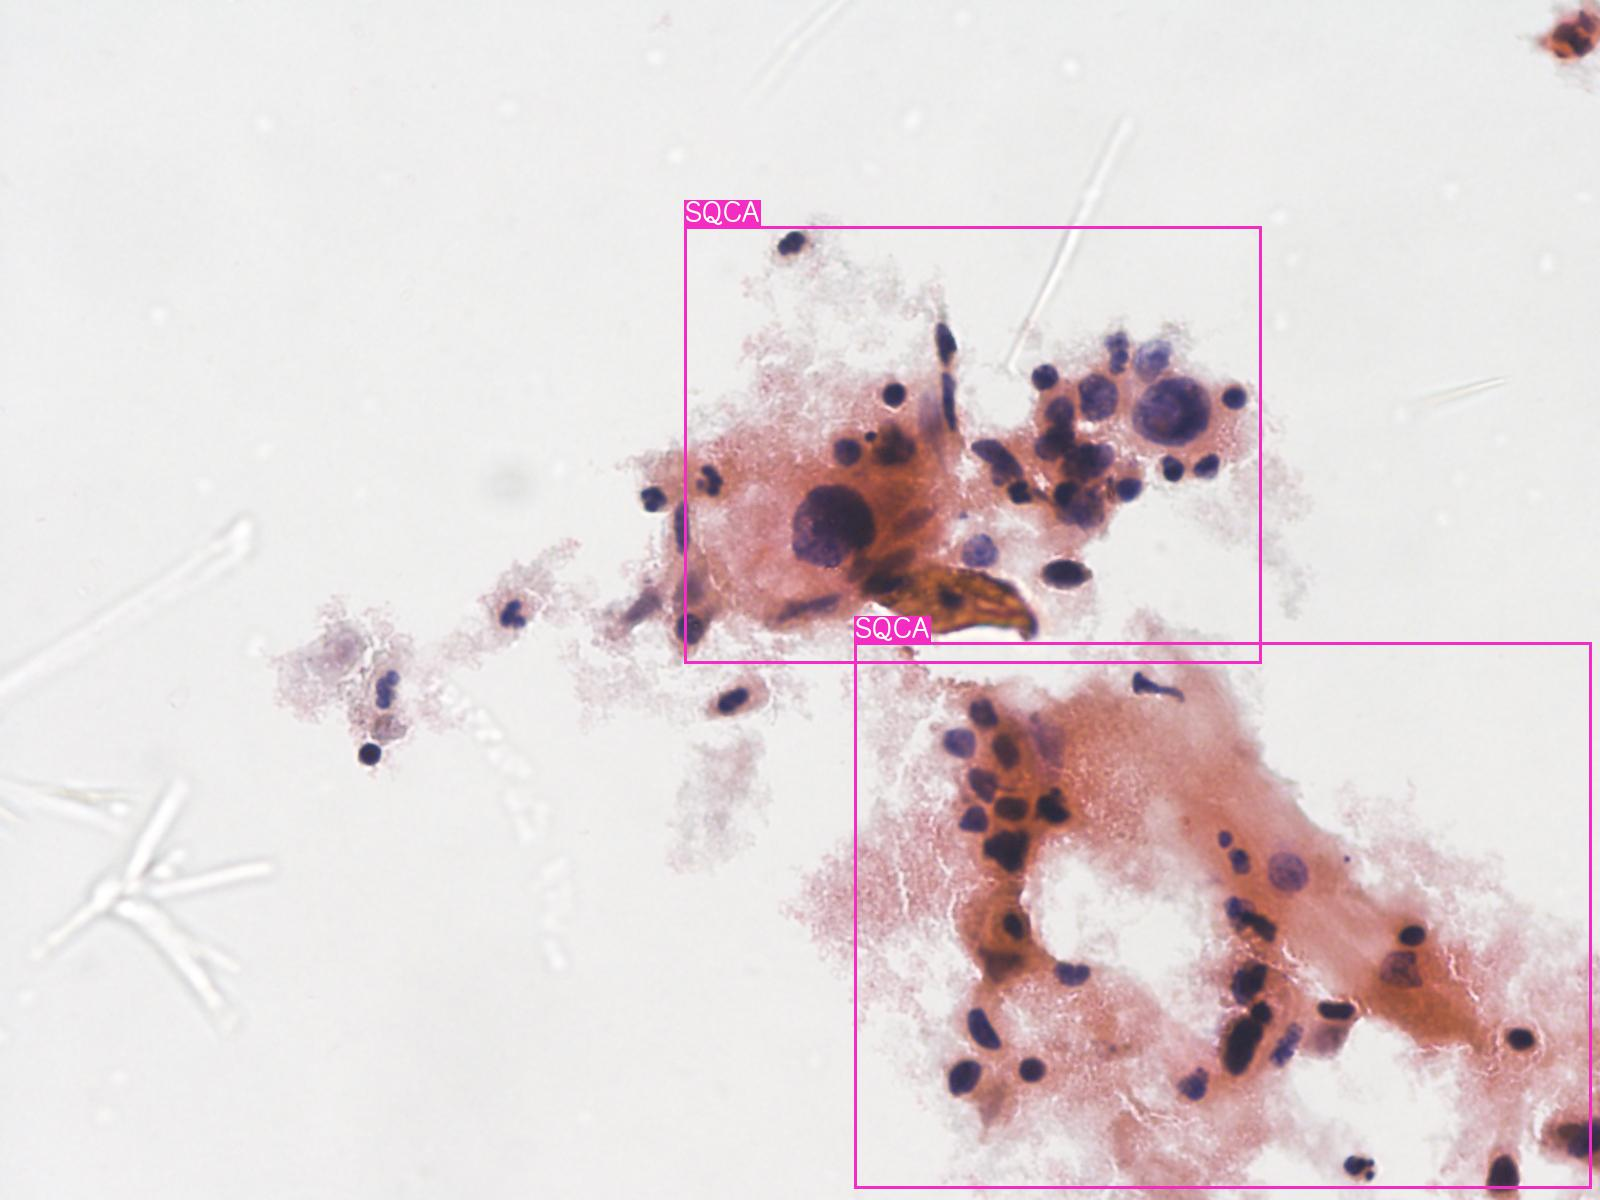
\includegraphics[width = .49\linewidth]{TCTDataSet/可视化2.jpg}
    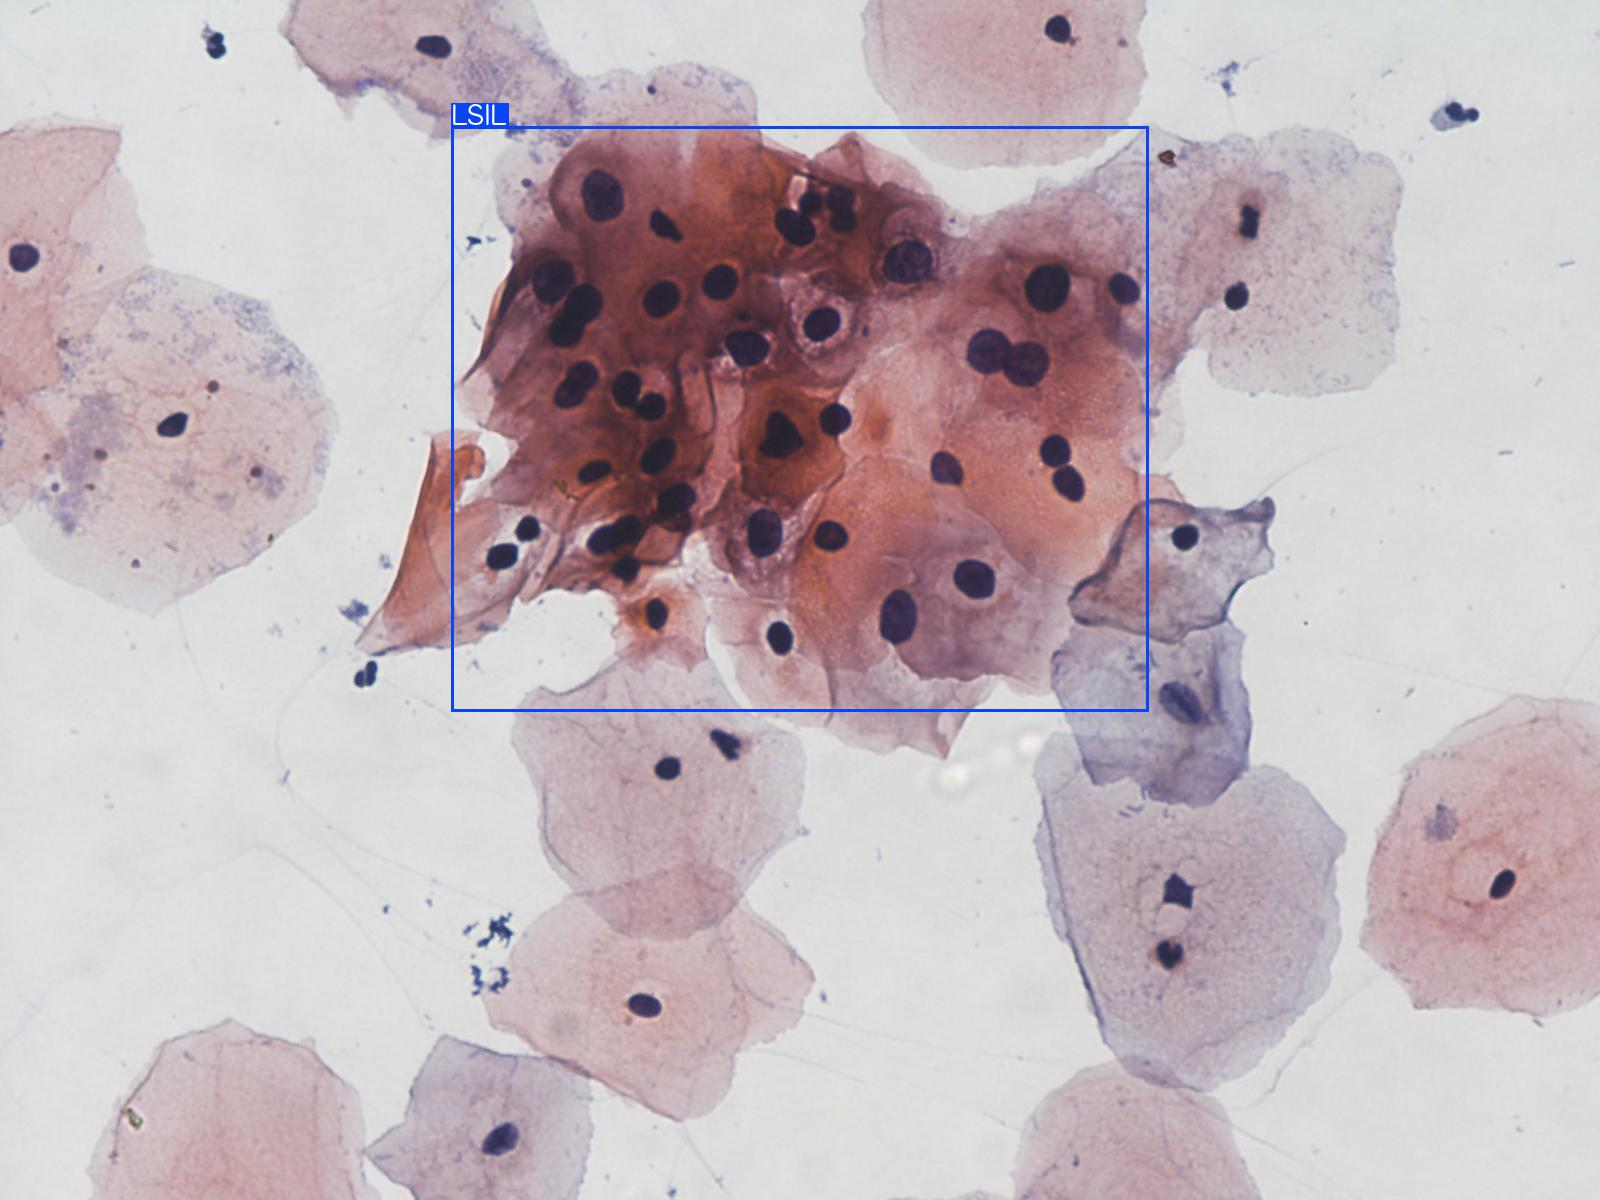
\includegraphics[width = .49\linewidth]{TCTDataSet/可视化3.jpg}
    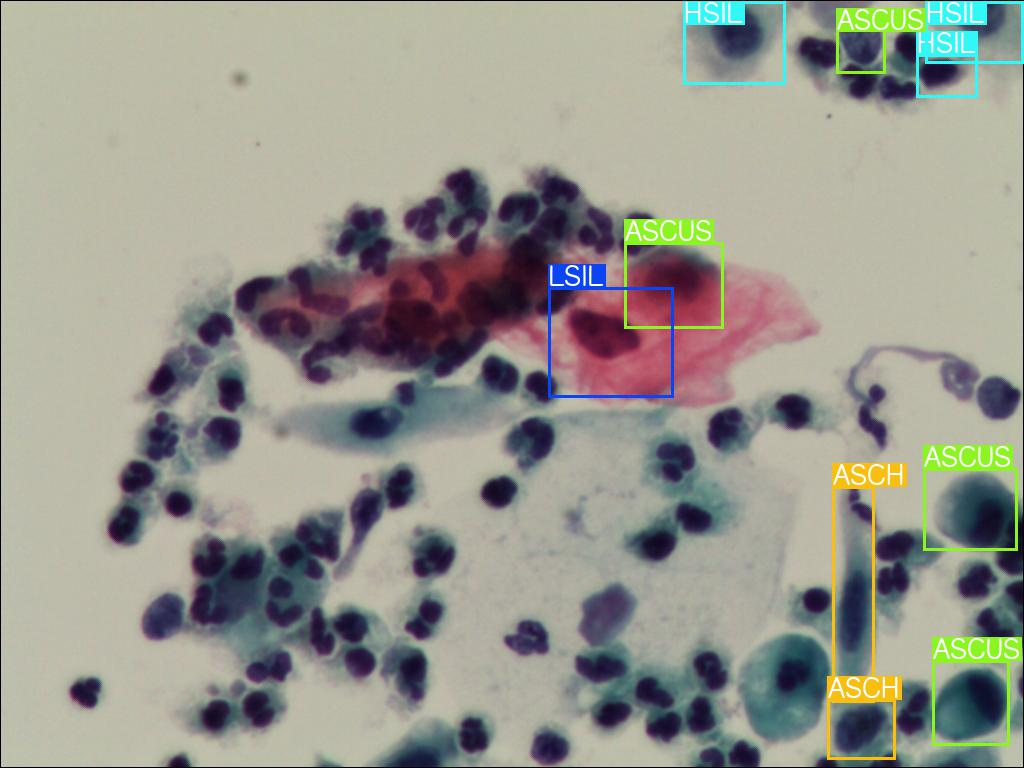
\includegraphics[width = .49\linewidth]{TCTDataSet/可视化4.jpg}
    \caption{部分数据集图片和标注框的可视化结果}
    \label{pic:数据集可视化}
\end{figure}

\section{方法}
\subsection{数据预处理与数据增强}
\subsubsection{放缩}
\par 我们首先将图片保持宽高比地放缩到不大于宽1333个像素,高800个像素的最大尺寸,例如,如果一张图片的大小是宽1024个像素,高720个像素,那么,如果将宽放大到1333个像素则会放大大约$1.3$倍,而如果将高放大到800个像素则会放大大约$1.11$倍,而$1.3>1.11$,因此,图片只能将高放大到800个像素,宽度放大到1138个像素。这样既保持了图片的宽高比没有被改变从而没有使图片变形,又保证了图片不会超过预订的尺寸可以被放入网络中进行计算。
\subsubsection{随机翻转}
\par 当我们每次从数据集中取出一张图片时,我们会有$50\%$的概率将这张图片进行水平的翻转,而另有$50\%$的概率将直接读取这张图片不做任何变化。
\subsubsection{正规化}
\par 我们会将数据集中的每张图片都做正规化处理再进行训练,这是指将图片中的每个像素的三个通道都减去平均值再除以相应的标准差,如公式\ref{eq:正规化预处理}所示。
\begin{equation}
    P_{i,j,c}=\frac{P_{i,j,c}-mean_{c}}{std_{c}}
    \label{eq:正规化预处理}
\end{equation}

\par 其中,$P_{i,j,c}$是指图片在$i,j$处$c$通道的值,$mean$和$std$都是三维的向量,分别表示三个通道在整个数据集上的平均值与标准差,其计算方式如公式\ref{eq:正规化参数}所示。
\begin{equation}
    \begin{aligned}
        mean_c&=\frac{\sum_{k=0}^N\frac{\sum_{i=0}^{H^k}\sum_{j=0}^{W^k}P_{i,j,c}^k}{H^k*W^k}}{N}\\
        std_c&=\sqrt{\frac{\sum_{k=0}^N\frac{\sum_{i=0}^{H^k}\sum_{j=0}^{W^k}(P_{i,j,c}^k-mean_c)^2}{H^k*W^k}}{N}}
    \end{aligned}
    \label{eq:正规化参数}
\end{equation}

\par 其中,$P_{i,j,c}^k$是指数据集中的第k张图片在$i,j$处$c$通道的值,$H^K$和$W^k$分别指第k张图片的高和宽,$N$是指数据集中共有$N$张图片。在本文中,$mean$与$std$变量的取值如\ref{eq:正规化参数取值}所示。
\begin{equation}
    \begin{aligned}
        mean&=[123.675, 116.28, 103.53]\\
        std&=[58.395, 57.12, 57.375]
    \end{aligned}
    \label{eq:正规化参数取值}
\end{equation}

\subsubsection{零填充}
\par 之后,我们会将图片填充到宽与高都是32的倍数,不足的像素点使用零来填充。
\subsection{任务分解}
\par 正如我们在\ref{par:单细胞与细胞簇的形态差异}中所提到的,医生在标注框的时候会遇到大片病变细胞粘连在一起因而无法区分开的情况,这时医生只能选择将整个细胞簇框住,因此,每个标注框就有了两个可能的含义——单个病变细胞或者整个的病变细胞簇,而这二者有着明显的形态差异与语义差异,因此,我们为这两种不同的任务设计了不同的检测头,通过让每个检测头分别检测不同的目标达到提高检测准确度的目的。
\par 最后,我们会使用额外的一个检测头综合前面两个检测头的检测结果并给出最终结果,这样的设计既让不同的网络部分分别完成不同的任务,减轻了网络学习的负担,提高了网络的检测精度,又可以充分的利用到整张图像上的整体信息,不会造成由于信息的缺失而导致的性能下降等问题。
\subsection{细胞对比}
\par 如我们在章节\ref{par:类别判定的主观性}中所提到的,医生在为标注框标注类别时可能会有较大的主观倾向性,而且由于病变是一个不断发展的过程,病变细胞在不断发展的过程中可能会刚好处于某两个类别之间的状况,这时的病变细胞会同时具有这两个类别的某些特征,这就会影响医生对细胞类别的判断,也会造成病变类别判断的模糊性与不明确性。因此,如何准确的判断检测到的病变细胞的类别是一个较大的困难,我们为此设计了多个模块帮助网络加强对病变细胞类别的判断。
\subsubsection{病变细胞关系模块}
\par 这一模块会将当前图片中所有的检测到的病变细胞的特征计算做一次两两之间的关系,并得到新的关系特征,如\ref{eq:关系计算}所示。

\begin{equation}
    \begin{aligned}
        W_R&=Softmax((FP)(FP)^T)\\
        F_R&=W_RF
    \end{aligned}
    \label{eq:关系计算}
\end{equation}

\par 其中,$F$是指病变细胞的特征,它是一个$N\times M$的矩阵,其中,$N$是当前图片中检测到的病变细胞的数量,$M$是每个病变细胞特征的维度,在本文中我们取$1024$。$P$是一个$M\times M$的矩阵,它表示将病变细胞的特征转化到某个编码空间中的编码方式,是一个可学习的参数。$W_R$表示病变细胞特征之间的关系权重。$F_R$表示计算得到的关系特征。
\subsubsection{特征差分模块}
\par 这一模块会将当前图片中所有的检测到的病变细胞的特征与检测到的正常细胞做特征差分运算。为此,我们的模型除去上述的三个检测头以外,还有一个专门用来检测正常细胞的检测头,如果在当前图片中检测到了正常细胞,那么我们将会把所有正常细胞的特征先做一次存储以备后用,然后从所有被检测到的正常细胞中挑选出最好的正常细胞的特征用于本次的差分运算。而如果当前图片中没有检测到正常细胞,我们就会从之前存储的正常细胞特征中随机地挑选出一个来用作差分计算。差分计算的方式如\ref{eq:差分计算}所示。

\begin{equation}
    \begin{aligned}
        F_D&=F_A-F_N
    \end{aligned}
    \label{eq:差分计算}
\end{equation}

\par 其中,$F_A$是指所有病变细胞的特征,$F_N$是指所使用的正常细胞的特征,正常细胞的特征会先被复制到与异常细胞的特征同等尺寸再做运算。$F_D$表示计算得到的差分特征。

\subsubsection{综合}
\par 当我们完成所有的特征计算之后我们会直接将关系特征、差分特征与初始的病变细胞的特征直接相加用作之后的检测,如\ref{eq:特征融合}所示。

\begin{equation}
    \begin{aligned}
        F_F&=F+F_R+F_D
    \end{aligned}
    \label{eq:特征融合}
\end{equation}

\par 其中,$F_F$是指最后计算得到的特征,$F$是指初始的病变细胞的特征,$F_R$是指关系计算得到的特征,$F_R$是指差分计算得到的特征。

\section{实验与结果}

\section{结论}

\section{研究展望}
